\documentclass[10pt,a4paper]{article}
\usepackage[utf8]{inputenc}
\usepackage{amsmath}
\usepackage{amsfonts}
\usepackage{amssymb}
\usepackage{graphicx}
\usepackage{lmodern}
\usepackage{graphicx}
\usepackage{array}
\usepackage{float}
\usepackage{xcolor}
\usepackage{listings}
\usepackage{color} %red, green, blue, yellow, cyan, magenta, black, white
\definecolor{mygreen}{RGB}{28,172,0} % color values Red, Green, Blue
\definecolor{mylilas}{RGB}{170,55,241}




\title{Statistique: \\Projet 1}
\author{Sauvage Mehdi}
\begin{document}

\lstset{language=Matlab,%
    %basicstyle=\color{red},
    breaklines=true,%
    morekeywords={matlab2tikz},
    keywordstyle=\color{blue},%
    morekeywords=[2]{1}, keywordstyle=[2]{\color{black}},
    identifierstyle=\color{black},%
    stringstyle=\color{mylilas},
    commentstyle=\color{mygreen},%
    showstringspaces=false,%without this there will be a symbol in the places where there is a space
    numbers=left,%
    numberstyle={\tiny \color{black}},% size of the numbers
    numbersep=9pt, % this defines how far the numbers are from the text
    emph=[1]{for,end,break},emphstyle=[1]\color{red}, %some words to emphasise
    %emph=[2]{word1,word2}, emphstyle=[2]{style},    
}




\maketitle
\newpage
\section{Analyse descriptive}



\subsection*{(a)}
\ \\

Vu l'allure des histogrammes, nous pouvons déduire que la question 1 était globalement mieux réussi que la question 2 et la question 3. La question 2 et la question 3 ont, quant à elles, été plus équitablement réparti entre les différentes cotes possibles. 
\ \\

\begin{figure}[h]
\centering
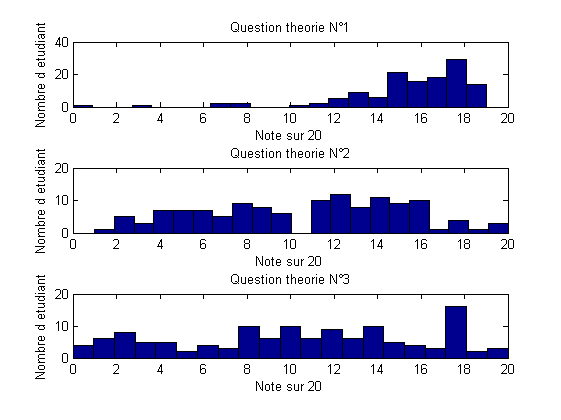
\includegraphics[scale= 0.5]{1a_graphe.png}
\end{figure}

\subsection*{(b)}
\ \\

Dans le tableau, ci-dessous, sont reprit les moyennes, médianes, modes et écarts-types des questions d'exercice:

\begin{center}
\begin{tabular}{|c|c|c|c|}
\hline
... & Question 1 & Question 2 & Question 3 \\
\hline
\hline
Moyennes & 11.9685 & 14.6614 & 6.5669 \\
\hline
Médianes & 12 & 16 & 5 \\
\hline
Modes & 20 & 19 & 0 \\
\hline
écarts-Types & 5.8580 & 4.5639 & 6.6781 \\
\hline

\end{tabular}
\end{center}
\ \\

Nous constatons que la question 2 a été bien mieux réalisée que les 2 autres. A la 1er question, les étudiants aillant eu 20 représentent la plus grande proportion alors que la moyenne n'est qu'à 11.96. Pour la question 2, la moyenne et la médiane sont plus élevées que pour la question 1 mais la plus grand partie des étudiants ont eu 19.
\ \\

Nous pouvons voir que la question 3 est la seule qui a en moyenne pas été réussi. En effet, une majorité des étudiants n'ont pas répondu à la question ou ont eu zero. En effet, la moyenne ne se situe qu'à 6.57. 
\ \\

Pour qu'un résultat soit estimé "Normal" au sens de la lois normal, il doit être tel que

\begin{center}
Donnée $\epsilon$ [Moyenne - Ecart-type ; Moyenne + Ecart-type] 
\end{center}
\ \\

Dés lors, pour qu'une donnée soit normal elle doit être comprise entre:

\begin{center}
\begin{tabular}{|c|c|c|c|}
\hline
... & Question 1 & Question 2 & Question 3 \\
\hline
\hline
Interval Normal & [6,12 ; 17.81] & [10,10 ; 19,22] & [-0.11 ; 13.25] \\
\hline
 Nbr Normal & 72 & 103 & 99 \\
\hline
 Proportion & 56,69\% & 81.11\% & 77.95\% \\
 
\hline
\end{tabular}
\end{center}

\subsection*{(c)}
\ \\ 

Comme nous pouvons observer dans les graphiques ci-dessous, il existe des données aberrantes pour les 2 projets et pour la question relative au projet. En effet, pour le projet 1 et 2 , certain étudiant on eu des cotes en dessous de 13 et en dessous de 10 alors que d'autres étudiants on eu 20 à la question du projet lors de l'examen. Toutes ces données constitue des aberrations statistiques.
\ \\

Notons que les valeurs aberrantes sont défini comme appartenant à:
\begin{center}
$[ q1 – 1.5 \times (q3 – q1) ; q3 + 1.5 \times (q3 – q1) ]$\\
 q1 and q3 sont les 25eme and 75eme quartiles des données.
\end{center}

\begin{figure}[h]
\centering
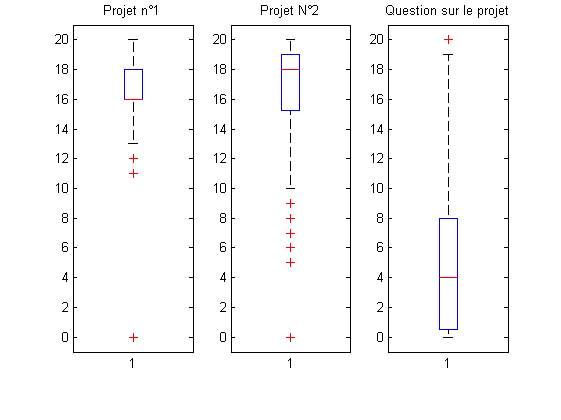
\includegraphics[scale= 0.5]{1c_graphe.png}
\end{figure}
 
\begin{center}
\begin{tabular}{|c|c|c|c|}
\hline
... & Projet 1 & Projet 2 & Question projet \\
\hline
\hline
quartile 25 & 16 & 15.25 & 0.5 \\
\hline
Médianes & 16 & 18 & 4 \\
\hline
quartile 75 & 18 & 19 & 8 \\
\hline
limite aberrance sup & 20 & 20 & 19.25 \\
\hline
limite aberrance inf & 13 & 10 & 0 \\
\hline


\end{tabular}
\end{center}
\ \\
 

\subsection*{(d)}

\begin{figure}[h]
\centering
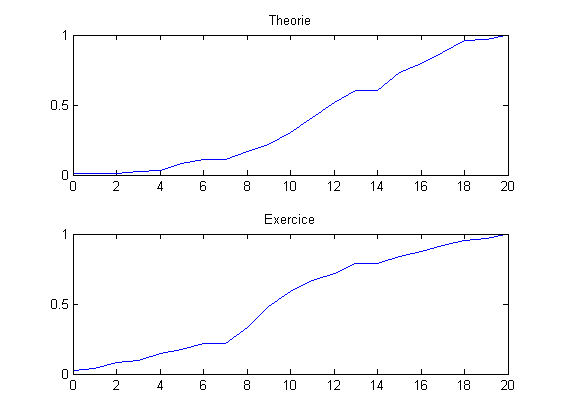
\includegraphics[scale= 0.5]{1d_graphe.png}
\end{figure}

\begin{center}
\begin{tabular}{|c|c|c|}
\hline
... & Theorie & Exercices \\
\hline
\hline
proportion de [10;14] & 0.3858 & 0.3071 \\
\hline
\end{tabular}
\end{center}
\ \\
 

\subsection*{(e)}
\ \\

Vu l'allure du graphe, nous ne pouvons pas tirer de relation évidente entre les deux données. Cette conclusion est appuyé par le coefficient de corrélation assez éloigné de 1.

le coefficient de corrélation est 0.2360.

\begin{figure}[h]
\centering
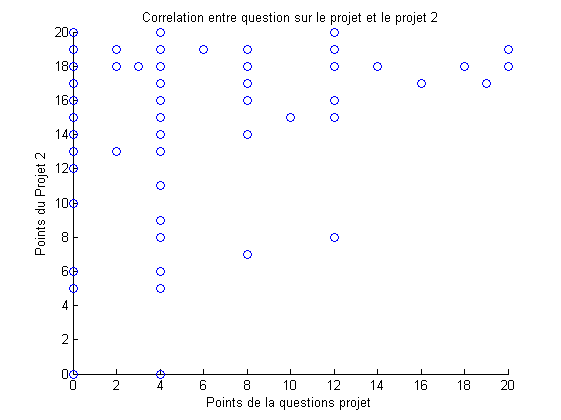
\includegraphics[scale= 0.5]{1e_graphe.png}
\end{figure}




\section{Génération d'échantillons i.i.d.}
\subsection*{(a)}
\subsubsection*{i}
\ \\

Nous pouvons constater que les moyennes, médianes et écarts-types calculées pour les échantillons ne sont pas très éloignées des mêmes valeurs pour la population entière. Néanmoins, ces valeurs pourraient s'en éloigner si l'échantillon considéré était moins représentatif de la population global. 

\begin{center}
\begin{tabular}{|c|c|c|c|}
\hline
... & Exercice 1 & Exercice 2 & Exercice 3 \\
\hline
\hline
Moyennes de l'échantillon  & 11.15 & 15 & 6.75 \\
\hline
Médianes de l'échantillon  & 10.5 & 16.5 & 5 \\
\hline
Ecart-types de l'échantillon & 4.86 & 4.71 & 6.92 \\
\hline

\end{tabular}
\end{center}
\ \\
 

\subsubsection*{ii}
\ \\

Ci-dessous ce trouve les boites à moustaches relative aux projets. 
Nous pouvons constater que même si les allures générales sont conservées, il y a des différences importantes entres les boites relative a l'échantillon et à la population global.  

\begin{figure}[h]
\centering
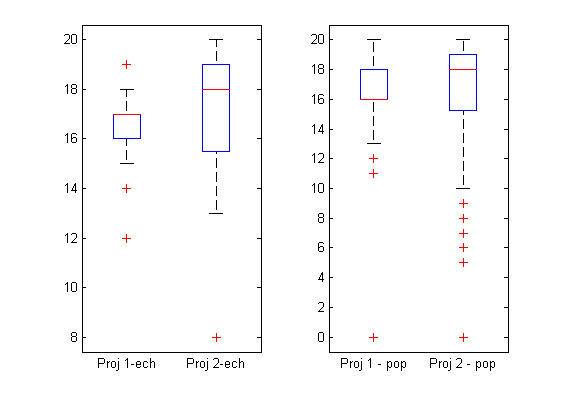
\includegraphics[scale= 0.5]{2aii_graphe.png}
\end{figure}



\subsubsection*{iii}
\ \\

Voici, ci-dessous, les polygones des fréquences cumulées relatif aux questions de théorie. 
\begin{figure}[h]
\centering
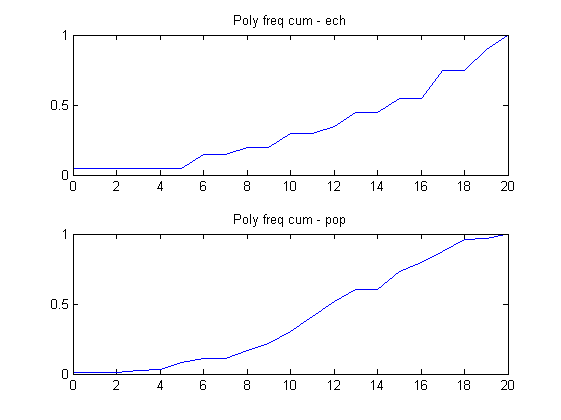
\includegraphics[scale= 0.5]{2aiii_graphe.png}
\end{figure}
\ \\

Comme constaté dans les questions précédentes, les allures générales sont conservées mais les détails des graphiques ne sont pas les mêmes.
\ \\ 

La distance de Kolmogorov Smirnov a été calculée comme cela:

\begin{center}

$max\{ abs\{$ vec$\_$freq$\_$cum(population) $-$ vec$\_$freq$\_$cum(echantillon)$\} \}$
\ \\

$ =0.2453$ 
\end{center}



\subsection*{(b)}
\ \\

Prenons $100$ échantillons de $20$ étudiants pour faire une moyenne des moyennes, médianes et écart-types des échantillons de la question 1 d'exercice. 
\ \\
 
Notons que les questions i , ii et iii ont pour résultat des graphiques aillant l'allure d'une gaussienne. En effet, ces données semble obéir à des lois Normales. 
\ \\

Pour ces trois mêmes questions, nous pouvons constaté que les moyennes des médianes, moyennes et écart-types prisent sur 100 échantillons sont beaucoup plus proche que lorsque que l'on ne considère qu'un seul échantillon. Cela semble logique puisque la population est mieux représenté par 100 sélections de 20 étudiants que une seule.


\subsubsection*{i}
\ \\

La moyenne des moyennes des échantillons est 12.04. Pour la population totale, la moyenne est de 11.96. 

\begin{figure}[H]
\centering
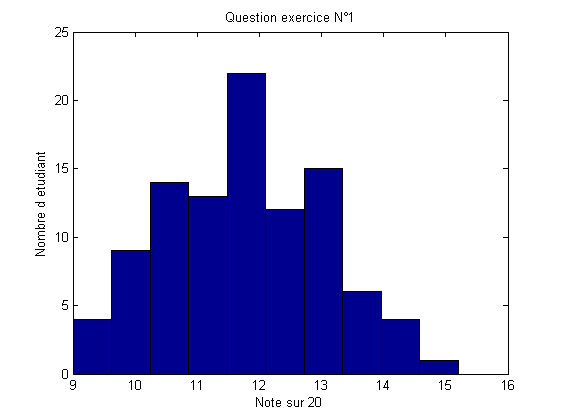
\includegraphics[scale= 0.5]{2bi_graphe.png}
\end{figure}
\ \\

\subsubsection*{ii}


La moyenne des médianes des échantillons est $12,33$ points. Pour la population totale, la médiane est de $12$ points. 

\begin{figure}[H]
\centering
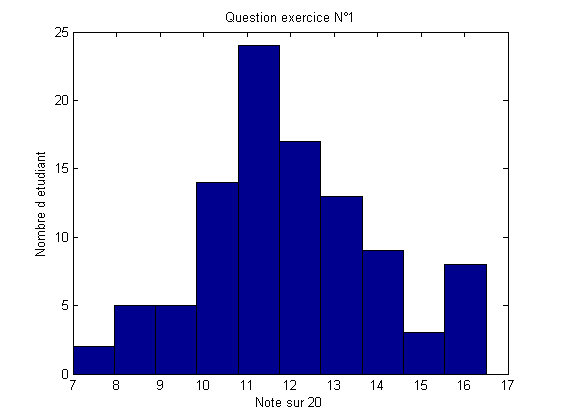
\includegraphics[scale= 0.5]{2bii_graphe.png}
\end{figure}
\ \\

\subsubsection*{iii}

La moyenne des écart-types des échantillons est $5.74$ points.Pour la population totale, l'écart-type est de $5.85$ points. 

\begin{figure}[H]
\centering
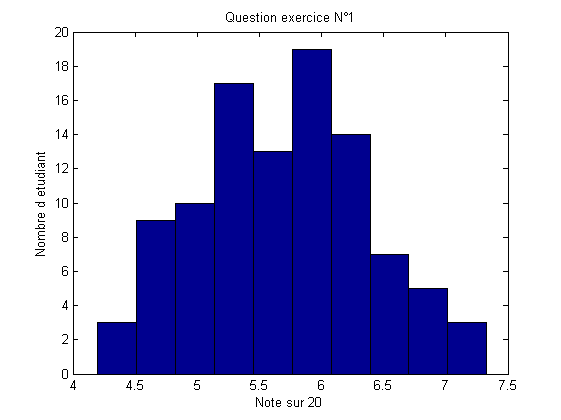
\includegraphics[scale= 0.5]{2biii_graphe.png}
\end{figure}
\ \\

\subsubsection*{iv et v}

Les trois histogramme ont la même allure et ressemble vaguement au graphique d'une lois de poisson. Ils croient rapidement jusqu'à un maximum au environ de 0.18 et puis diminue plus doucement jusque qu'a arriver a 0. 
\ \\

La lois de poisson est construite en se basant sur l'idée que la distance de Kolmogorov Smirnov la plus fréquente ce situe vers 0.18 mais il est plus naturelle de trouver des distance plus petite car les 100 echantillons représente relativement bien la population. Au dela de 0.18, il y a une brusque diminution du nombre d'étudiant car la l'échantillon devrait , en général, donner une distance de Kolmogorov Smirnov plus petite.
\begin{figure}[H]
\centering
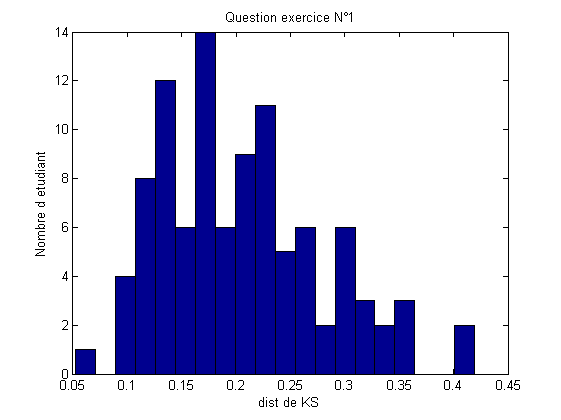
\includegraphics[width=6cm]{2biv_graphe.png} \hfill
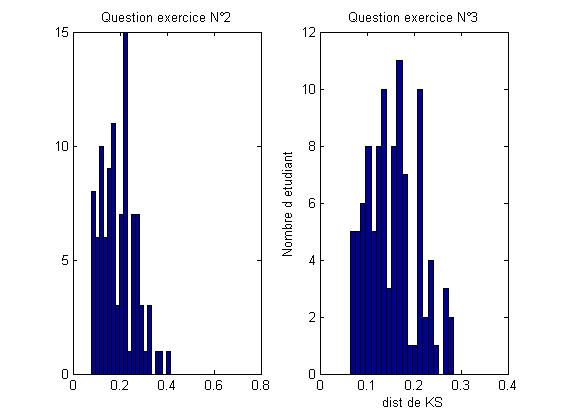
\includegraphics[width=6cm]{2bv_graphe.png}
\end{figure}
\ \\

\newpage

\section*{Code}

\lstinputlisting{Q1a.m}
\newpage
\lstinputlisting{Q1b.m}
\newpage
\lstinputlisting{Q1c.m}
\newpage
\lstinputlisting{Q1d.m}
\newpage
\lstinputlisting{Q1e.m}
\newpage
\lstinputlisting{Q2ai.m}
\lstinputlisting{Q2aii.m}
\newpage
\lstinputlisting{Q2aiii.m}
\newpage
\lstinputlisting{Q2bi.m}
\lstinputlisting{Q2bii.m}
\newpage
\lstinputlisting{Q2biii.m}
\lstinputlisting{Q2biv.m}
\newpage
\lstinputlisting{Q2bv.m}

\end{document}